%%%%%%%%%%%%%%%%%%%%%%%%%%%%%%%%%%%%%%%%%
% Journal Article
% LaTeX Template
% Version 1.3 (9/9/13)
%
% This template has been downloaded from:
% http://www.LaTeXTemplates.com
%
% Original author:
% Frits Wenneker (http://www.howtotex.com)
%
% License:
% CC BY-NC-SA 3.0 (http://creativecommons.org/licenses/by-nc-sa/3.0/)
%
%%%%%%%%%%%%%%%%%%%%%%%%%%%%%%%%%%%%%%%%%

%----------------------------------------------------------------------------------------
%	PACKAGES AND OTHER DOCUMENT CONFIGURATIONS
%----------------------------------------------------------------------------------------

\documentclass{article}

%\documentclass{aastex}  % version 5.0 or prior
%\usepackage{natbib}



\usepackage{graphicx}
\usepackage{lipsum} % Package to generate dummy text throughout this template
%\usepackage[sc]{mathpazo} % Use the Palatino font
\usepackage[T1]{fontenc} % Use 8-bit encoding that has 256 glyphs
\linespread{1.05} % Line spacing - Palatino needs more space between lines
\usepackage{microtype} % Slightly tweak font spacing for aesthetics

\usepackage[margin=1in,columnsep=20pt]{geometry} % Document margins
\usepackage{multicol} % Used for the two-column layout of the document
\usepackage[hang, small,labelfont=bf,up,textfont=it,up]{caption} % Custom captions under/above floats in tables or figures
\usepackage{booktabs} % Horizontal rules in tables
\usepackage{float} % Required for tables and figures in the multi-column environment - they need to be placed in specific locations with the [H] (e.g. \begin{table}[H])
\usepackage{hyperref} % For hyperlinks in the PDF
\usepackage{subcaption}

\usepackage{lettrine} % The lettrine is the first enlarged letter at the beginning of the text
\usepackage{paralist} % Used for the compactitem environment which makes bullet points with less space between them
\usepackage{amsmath}
\usepackage{abstract} % Allows abstract customization
\renewcommand{\abstractnamefont}{\normalfont\bfseries} % Set the "Abstract" text to bold
\renewcommand{\abstracttextfont}{\normalfont\small\itshape} % Set the abstract itself to small italic text

\usepackage{titlesec} % Allows customization of titles
%\renewcommand\thesection{\Roman{section}} % Roman numerals for the sections
%\renewcommand\thesubsection{\Roman{subsection}} % Roman numerals for subsections
%\renewcommand\thesubsubsection{\Alph{subsubsection}} % Roman numerals for subsections
\titleformat{\section}[block]{\Large\scshape}{\thesection}{1em}{} % Change the look of the section titles
\titleformat{\subsection}[block]{\large}{\thesubsection}{1em}{} % Change the look of the section titles
\titleformat{\subsubsection}[block]{}{\thesubsubsection}{1em}{} % Change the look of the section titles

\usepackage{fancyhdr} % Headers and footers
\pagestyle{fancy} % All pages have headers and footers
\fancyhead{} % Blank out the default header
\fancyfoot{} % Blank out the default footer
\fancyhead[C]{Montana State University \quad $\bullet$ \quad CSCI 466 Artificial Intelligence \quad $\bullet$ \quad Group 21} % Custom header text
\fancyfoot[RO,LE]{\thepage} % Custom footer text

\newcommand{\ve}[1]{\boldsymbol{\mathbf{#1}}}

%----------------------------------------------------------------------------------------
%	TITLE SECTION
%----------------------------------------------------------------------------------------

\title{\vspace{-15mm}\fontsize{24pt}{10pt}\selectfont\textbf{CSCI 446 Artificial Intelligence \\ Project 1 Final Report} \\[-2mm]} % Article title
\date{\today}
\author{
\large
\textsc{Roy Smart} \and \textsc{Nevin Leh} \and \textsc{Brian Marsh}\\[2mm] % Your name
}


%----------------------------------------------------------------------------------------

\begin{document}

\maketitle % Insert title

\thispagestyle{fancy} % All pages have headers and footers

%\begin{abstract}
%We present a novel way of performing MOSES data inversions using a
%\end{abstract}

%----------------------------------------------------------------------------------------
%	ARTICLE CONTENTS
%----------------------------------------------------------------------------------------

%\begin{multicols}{2} % Two-column layout throughout the main article text
\normalsize
\section{Introduction}
	The \textit{Graph Coloring Problem} (GCP) is the problem of attempting to color a set of interconnected vertices, using a limited set of colors, such that no vertex has the same color as its neighbors. This problem is best visualized as the map coloring problem. As an example of the map coloring problem, consider the problem of assigning one of four colors to every country in the world, such that no two adjacent countries have the same color, as in Figure \ref{world}. 
	\begin{figure}[h!]
		\centering
		\includegraphics[width=0.8\textwidth]{images/world_map}
		\caption{Map of the world satisfying the map coloring problem \cite{world}.}
		\label{world}
	\end{figure}
	It can be shown that the map coloring problem reduces to the graph coloring problem\cite{ai} if we represent the countires as the vertices of the graph, and the borders between countries as the edges of the graph, shown in Figure \ref{four_col}. This configuration produces a \textit{planar} graph, a graph with no edge intersections. 	
	\begin{figure}[h!]
		\centering
		\includegraphics[width=0.8\textwidth]{images/four_color}
		\caption{Diagram describing how the map coloring problem can be transformed into the graph coloring problem \cite{four_color}.}
		\label{four_col}
	\end{figure}
	For this project, we are asked to solve the GCP problem for planar graphs only. Since the problems are guaranteed to be planar, we will represent our graphs using polygon maps generated by our program.
	
	To solve the GCP we employed five different algorithms: Minimum Conflicts, Simple Backtracking, Backtracking with Forward Checking, Backtracking with Constraint Propagation (MAC), and Local Search using a Genetic Algorithm. To evaluate these algorithms, we built a problem generating program that can produce a random set of planar graphs. Using the problem generator, we calculated a set of graphs between the sizes \{10, 20, 30,...,100\} and called the five graph coloring algorithms to solve the GCP. We measured GCP algorithm performance by measuring the number of read/write operations, the time required to find a solution, and the number of function calls for each algorithm. Using these metrics, we predict that the Minimum Conflicts algorithm will be the fastest, based off its performance on the eight-queens problem\cite{ai}.


\par The code for this project is implemented in \texttt{C++} and depends on the programs \texttt{cairo}, \texttt{gnuplot}, \texttt{ffmpeg}, and \LaTeX \space for graph output, performance output, video output, and documentation respectively.


\section{Problem Generation}
	We created a function that could produce many examples of planar graphs from a set of randomly scattered points. For an arbitrary set of points, there is no unique planar graph that can be constructed. To solve this issue, the problem statement has provided a algorithm for calculating an planar graph. 
	\begin{quote}
	Select some point $X$ at random and connect $X$ by a straight line
	to the nearest point $Y$ such that $X$ is not already connected to $Y$ and line crosses no other line. Repeat the
	previous step until no more connections are possible.
	\end{quote}
	For our implementation of the above algorithm, we started by creating a complete graph (where each vertex is connected to every other vertex). Each vertex was associated with a list of edges, sorted by length. 
	We then selected a point at random and inspected the first unchecked edge $E$. If $E$ did not cross any of the accepted edges, it is added to the list of accepted edges and marked as checked. This process was repeated until every edge was marked as checked. \par
	The most challenging part of the implementation described above was determining if two line segments intersected. An algorithm to determine if two edges (or line segments) cross has been outlined by LaMothe \cite{tricks} and described in detail here. Let's start by defining two line segments 
	\begin{align}
		\begin{split}
			& A = \{ \ve{a},\; \ve{a'} \} \\
			& B = \{\ve{b}, \;\ve{b'}\}
		\end{split}
	\end{align}
	where $\ve{a}, \; \ve{a'}, \; \ve{b}, \text{ and } \ve{b'}$ are vectors from the origin to the ends of the line segments. Next, compute the direction vectors for each line segment
	\begin{align}
		\begin{split}
			&\ve{\alpha} = \ve{a}' - \ve{a} \\
			&\ve{\beta} = \ve{b}' - \ve{b} 
		\end{split}
	\end{align}
	Now, the trick to solving this problem is to parameterize the line segment using the direction vector and a parameter $t_i$ in the domain $[0, \; 1]$.
	\begin{align}
		\begin{split}
			& \ve{p} = \ve{a} + \ve{\alpha} t_a, \quad t_a \in [0, \; 1]\\
			& \ve{q} = \ve{b} + \ve{\beta} t_b, \quad t_b \in [0, \; 1]
		\end{split}
	\end{align}
	From here, the solution is obvious. To find the point of intersection, we set $\ve{p} = \ve{q}$ and solve for the values of $t_a$ and $t_b$. Then, if the solution is outside the domain of $t_i$, the line segments do not intersect. Thus,
	\begin{align}
		\Rightarrow \; &\begin{cases}
			p_x = q_x \\
			p_y = q_y
		\end{cases} \\
		\Rightarrow \; & \begin{cases}
			a_x + \alpha_x t_a = b_x + \beta_x t_b \\
			a_y + \alpha_y t_a = b_y + \beta_y t_b.
		\end{cases} \label{system}	
	\end{align}
	Equation \ref{system} is a system of two equations and two unknowns, solving for $t_a$ and $t_b$ gives
	\begin{align}
		\begin{split}
			&t_a = \frac{(-a_y + b_y)\beta_x + (a_x - b_x)\beta_y}{\alpha_y \beta_x - \alpha_x \beta_y} \\
			&t_b = \frac{(a_y - b_y)\alpha_x + (-a_x + b_x)\alpha_y}{-\alpha_y \beta_x + \alpha_x \beta_y}.
		\end{split} \label{final_expr}
	\end{align}
	Finally, we can determine whether $A$ and $B$ intersect if $0 < t_a < 1$ and $0 < t_b < 1$ evaluates to true. This method may be more inefficient than other algorithms, such as the example outlined by Cormen\cite{structs} due to the division operation in Equation \ref{final_expr}. \par 
	Using the expression above to determine line intersections, we were able to implement a problem generator that was reasonably efficient, generating approximately $1\times10^3$ examples per second. This efficiency was important, because it made testing and debugging the GCP algorithms much faster. Example output from the problem generator is shown in Figure \ref{pgen}.
	
	\begin{figure}[h!]
		\centering
		\begin{subfigure}{0.45\textwidth}
			\centering
			\includegraphics[width=\textwidth]{images/pgen}
			\caption{Planar graph with 100 vertices.}
			\label{pgen}
		\end{subfigure}
		\qquad
		\begin{subfigure}{0.45\textwidth}
			\centering
				\includegraphics[width=\textwidth]{images/pgen_poly}
				\caption{Polygon map corresponding to (a).}
				\label{pgen_poly}
		\end{subfigure}
		\caption{Visualization of the output of the problem generator. First a planar graph was created (a), and then a corresponding polygon map was found (b).}
	\end{figure}
	
	We have also implemented a way to produce a map of regions that is analogous to the graphs created by the problem generator, shown in Figure \ref{pgen_poly}.  
	Since the graph coloring problem does not uniquely define the map coloring problem, we had to invent a metric that produces appropriate graphs. To define our metric, consider that if a polygon $G_i$ corresponding to each point $P_i$ were constructed out of the midpoints $M_{i,m}$ of the associated edges $E_{i,m}$ of $P_i$, then an adjacent polygon $G_j$ would only touch at the corners, that is, our map would be full of gaps. Therefore, to fix the problem we also define the centroid $C_{i,n}$ of each triangle $T_{i,n}$ formed by the two adjacent edges $E_{i,m}$ and $E_{i,m+1}$. We then define the final polygon for $P_i$ using the points $M_{i,m}$ and $C_{i,n}$. This procedure is unnecessary in terms of the assignment, but is helpful for debugging GCP algorithms, demonstrating example output, and for aesthetic pleasure.
		
\section{Minimum Conflicts}
	
\section{Simple Backtracking}
	\subsection{Description}
		Backtracking is a method of solving constraint satisfaction problems through an "educated" exhaustive search. It works by building a partial solution one component at a time and then testing the solution to check if the solution still has a chance of success \cite{Golomb}. If the solution cannot possibly succeed, the algorithm \textit{backtracks} by moving back one component, modifying the component to form a new partial solution and then continuing. By checking partial solutions, backtracking can eliminate large portions of the solution-space, thus increasing the efficiency of the search.
		
		In the graph coloring problem, backtracking assigns colors to one vertex at a time and checks to see if it has the same value as any of its neighbors. If none of the possible colors work for the current vertex, it backs up and tries a different color on a previously assigned vertex. If a color has no conflicts, backtracking continues to the next vertex in the sequence.
		
		\begin{figure}[h!]
			\begin{subfigure}{0.18\textwidth}
				\centering
				\includegraphics[width=\textwidth]{images/sequences/simple_backtracking/bt_simple_I00001}
				\caption{}
				\label{bta}
			\end{subfigure}
			\;
			\begin{subfigure}{0.18\textwidth}
				\centering
				\includegraphics[width=\textwidth]{images/sequences/simple_backtracking/bt_simple_I00002}
				\caption{}
				\label{btb}
			\end{subfigure}
			\;
			\begin{subfigure}{0.18\textwidth}
				\centering
				\includegraphics[width=\textwidth]{images/sequences/simple_backtracking/bt_simple_I00004}
				\caption{}
				\label{btc}
			\end{subfigure}
			\;
			\begin{subfigure}{0.18\textwidth}
				\centering
				\includegraphics[width=\textwidth]{images/sequences/simple_backtracking/bt_simple_I00006}
				\caption{}
				\label{btd}
			\end{subfigure}
			\;
			\begin{subfigure}{0.18\textwidth}
				\centering
				\includegraphics[width=\textwidth]{images/sequences/simple_backtracking/bt_simple_I00007}
				\caption{}
				\label{bte}
			\end{subfigure} \\
			
			\begin{subfigure}{0.18\textwidth}
				\centering
				\includegraphics[width=\textwidth]{images/sequences/simple_backtracking/bt_simple_I00009}
				\caption{}
				\label{bta}
			\end{subfigure}
			\;
			\begin{subfigure}{0.18\textwidth}
				\centering
				\includegraphics[width=\textwidth]{images/sequences/simple_backtracking/bt_simple_I00012}
				\caption{}
				\label{btb}
			\end{subfigure}
			\;
			\begin{subfigure}{0.18\textwidth}
				\centering
				\includegraphics[width=\textwidth]{images/sequences/simple_backtracking/bt_simple_I00015}
				\caption{}
				\label{btc}
			\end{subfigure}
			\;
			\begin{subfigure}{0.18\textwidth}
				\centering
				\includegraphics[width=\textwidth]{images/sequences/simple_backtracking/bt_simple_I00019}
				\caption{}
				\label{btd}
			\end{subfigure}
			\;
			\begin{subfigure}{0.18\textwidth}
				\centering
				\includegraphics[width=\textwidth]{images/sequences/simple_backtracking/bt_simple_I00024}
				\caption{}
				\label{bte}
			\end{subfigure}

			\caption{A map coloring example using simple backtracking on an N=10 graph up to the first backtrack event. In panels (a) through (i), each vertex is assigned the first available color in the order (red, green, blue, pink).  Once the first pink assignment is made in panel (i), there are no possibilities remaining for the final vertex. The algorithm then backtracks and changes the node assigned in (h) to pink and tries again.}
			\label{bt_simple_ex}
		\end{figure}	
		
		
		
		
		
		
		To implement simple backtracking we followed the recursive algorithm outlined in Russel and Norvig Section 6.3 \cite{ai}. Russel's \textsc{Backtrack} loops through each value in the domain, and if the value is consistent with the constraints it recursively calls \textsc{Backtrack}. The function returns \texttt{true} when every variable has been assigned, and \texttt{false} if it cannot satisfy the constraints. The recursive function is advantageous, as it saves the state of the stack before each recursive call, making it trivial to restore the state of the solution after a failed recursive call to backtracking. 
		
		The crux of the backtracking procedure in the graph coloring problem is checking whether a coloring is consistent with constraints. From profiling our code, it was obvious that a fast constraint checking function was critical to the ability of backtracking to solve graph coloring problems up to $N=100$ vertices in a reasonable amount of time. This facilitated a change of design from an object-oriented approach, to an array-based approach.
	\subsection{Experimental Approach}
		To evaluate backtracking's performance on the graph coloring problem, we ran the algorithm on ten graph sizes $N=(10,\;20,\;...,\;100)$ with 20 trials for each value, for a total of 200 backtracking experiments. From each experiment we recorded the number of vertex reads, vertex writes, and number of recursive calls. Time constraints on this project demanded that we set a limit on the number of calls to backtracking, therefore we also recorded if this limit was reached for each experiment. 
		
		We expect that the number of recursive calls and the number of vertex writes and the number of vertex reads to be correlated by some constant factor. This is because there is a maximum of two writes and $N$ reads for each recursive call. Therefore, we can use this information to verify that the algorithm is working properly.
		
	
	\subsection{Results}
		
		\begin{figure}[h!]
			\centering
%			\includegraphics[width=0.8\textwidth]{../results_3/backtracking_simple/bt_simple_performance}
			\caption{Logarithmic plot describing the performance of the backtracking algorithm vs. the number of vertices. The shaded regions represent the minimum and maximum values of each quantity.}
		\end{figure}
	
\section{Backtracking with Forward Checking}

	\subsection{Description}
	
		Backtracking with forward checking incorporates the usual simple backtracking algorithm described in the preceding section, while incorporating an ability to look into the future to see if a particular assignment would create an inconsistency. Forward checking achieves this by trying to make an inconsistency occur as fast as possible by checking if all current assignments are consistent with each other \cite{haralick}.
		
		To accomplish forward checking in the graph coloring problem, we need to modify our representation of the graph to allow superpositions of colors and initialize the graph such that all colors are possible for each vertex. Next, for each call to backtracking, we assign a color to the next vertex, and delete that color from the vertex's neighbors list of possible colors. If any vertex has its list of possible colors completely eliminated, the algorithm backtracks and changes a color further up the tree.\cite{ai}.
		
		\begin{figure}[h!]
			\begin{subfigure}{0.18\textwidth}
				\centering
				\includegraphics[width=\textwidth]{images/sequences/forward_backtracking/bt_forward_I00003}
				\caption{}
				\label{bta}
			\end{subfigure}
			\;
			\begin{subfigure}{0.18\textwidth}
				\centering
				\includegraphics[width=\textwidth]{images/sequences/forward_backtracking/bt_forward_I00005}
				\caption{}
				\label{btb}
			\end{subfigure}
			\;
			\begin{subfigure}{0.18\textwidth}
				\centering
				\includegraphics[width=\textwidth]{images/sequences/forward_backtracking/bt_forward_I00007}
				\caption{}
				\label{btc}
			\end{subfigure}
			\;
			\begin{subfigure}{0.18\textwidth}
				\centering
				\includegraphics[width=\textwidth]{images/sequences/forward_backtracking/bt_forward_I00009}
				\caption{}
				\label{btd}
			\end{subfigure}
			\;
			\begin{subfigure}{0.18\textwidth}
				\centering
				\includegraphics[width=\textwidth]{images/sequences/forward_backtracking/bt_forward_I00011}
				\caption{}
				\label{bte}
			\end{subfigure} \\
			
			\begin{subfigure}{0.18\textwidth}
				\centering
				\includegraphics[width=\textwidth]{images/sequences/forward_backtracking/bt_forward_I00013}
				\caption{}
				\label{bta}
			\end{subfigure}
			\;
			\begin{subfigure}{0.18\textwidth}
				\centering
				\includegraphics[width=\textwidth]{images/sequences/forward_backtracking/bt_forward_I00015}
				\caption{}
				\label{btb}
			\end{subfigure}
			\;
			\begin{subfigure}{0.18\textwidth}
				\centering
				\includegraphics[width=\textwidth]{images/sequences/forward_backtracking/bt_forward_I00017}
				\caption{}
				\label{btc}
			\end{subfigure}
			\;
			\begin{subfigure}{0.18\textwidth}
				\centering
				\includegraphics[width=\textwidth]{images/sequences/forward_backtracking/bt_forward_I00019}
				\caption{}
				\label{btd}
			\end{subfigure}
			\;
			\begin{subfigure}{0.18\textwidth}
				\centering
				\includegraphics[width=\textwidth]{images/sequences/forward_backtracking/bt_forward_I00021}
				\caption{}
				\label{bte}
			\end{subfigure}
	
			\caption{The map coloring example from Figure \ref{bt_simple_ex} using backtracking with forward checking on an N=10 graph up to the first backtrack event. In panels (a) through (g), each vertex is assigned the first available color in the order (red, green, blue, pink), and deletes that color from the possible color of its neighbors. In panel (h) blue is assigned to the node on the left side, leaving two of its neighbors with only pink in their domain. Next, in panel (h), the central vertex has its domain reduced to the empty set, prompting a backtrack to panel (j). Note that forward checking in this case did not provide any advantage over backtracking.}
		\end{figure}
		

	\subsection{Experimental Approach}
	
	\subsection{Results}
	
\section{Backtracking with Constraint Propagation}

	\subsection{Description}
	
		\begin{figure}[h!]
			\begin{subfigure}{0.18\textwidth}
				\centering
				\includegraphics[width=\textwidth]{images/sequences/mac_backtracking/bt_mac_I00003}
				\caption{}
				\label{bta}
			\end{subfigure}
			\;
			\begin{subfigure}{0.18\textwidth}
				\centering
				\includegraphics[width=\textwidth]{images/sequences/mac_backtracking/bt_mac_I00004}
				\caption{}
				\label{btb}
			\end{subfigure}
			\;
			\begin{subfigure}{0.18\textwidth}
				\centering
				\includegraphics[width=\textwidth]{images/sequences/mac_backtracking/bt_mac_I00006}
				\caption{}
				\label{btc}
			\end{subfigure}
			\;
			\begin{subfigure}{0.18\textwidth}
				\centering
				\includegraphics[width=\textwidth]{images/sequences/mac_backtracking/bt_mac_I00008}
				\caption{}
				\label{btd}
			\end{subfigure}
			\;
			\begin{subfigure}{0.18\textwidth}
				\centering
				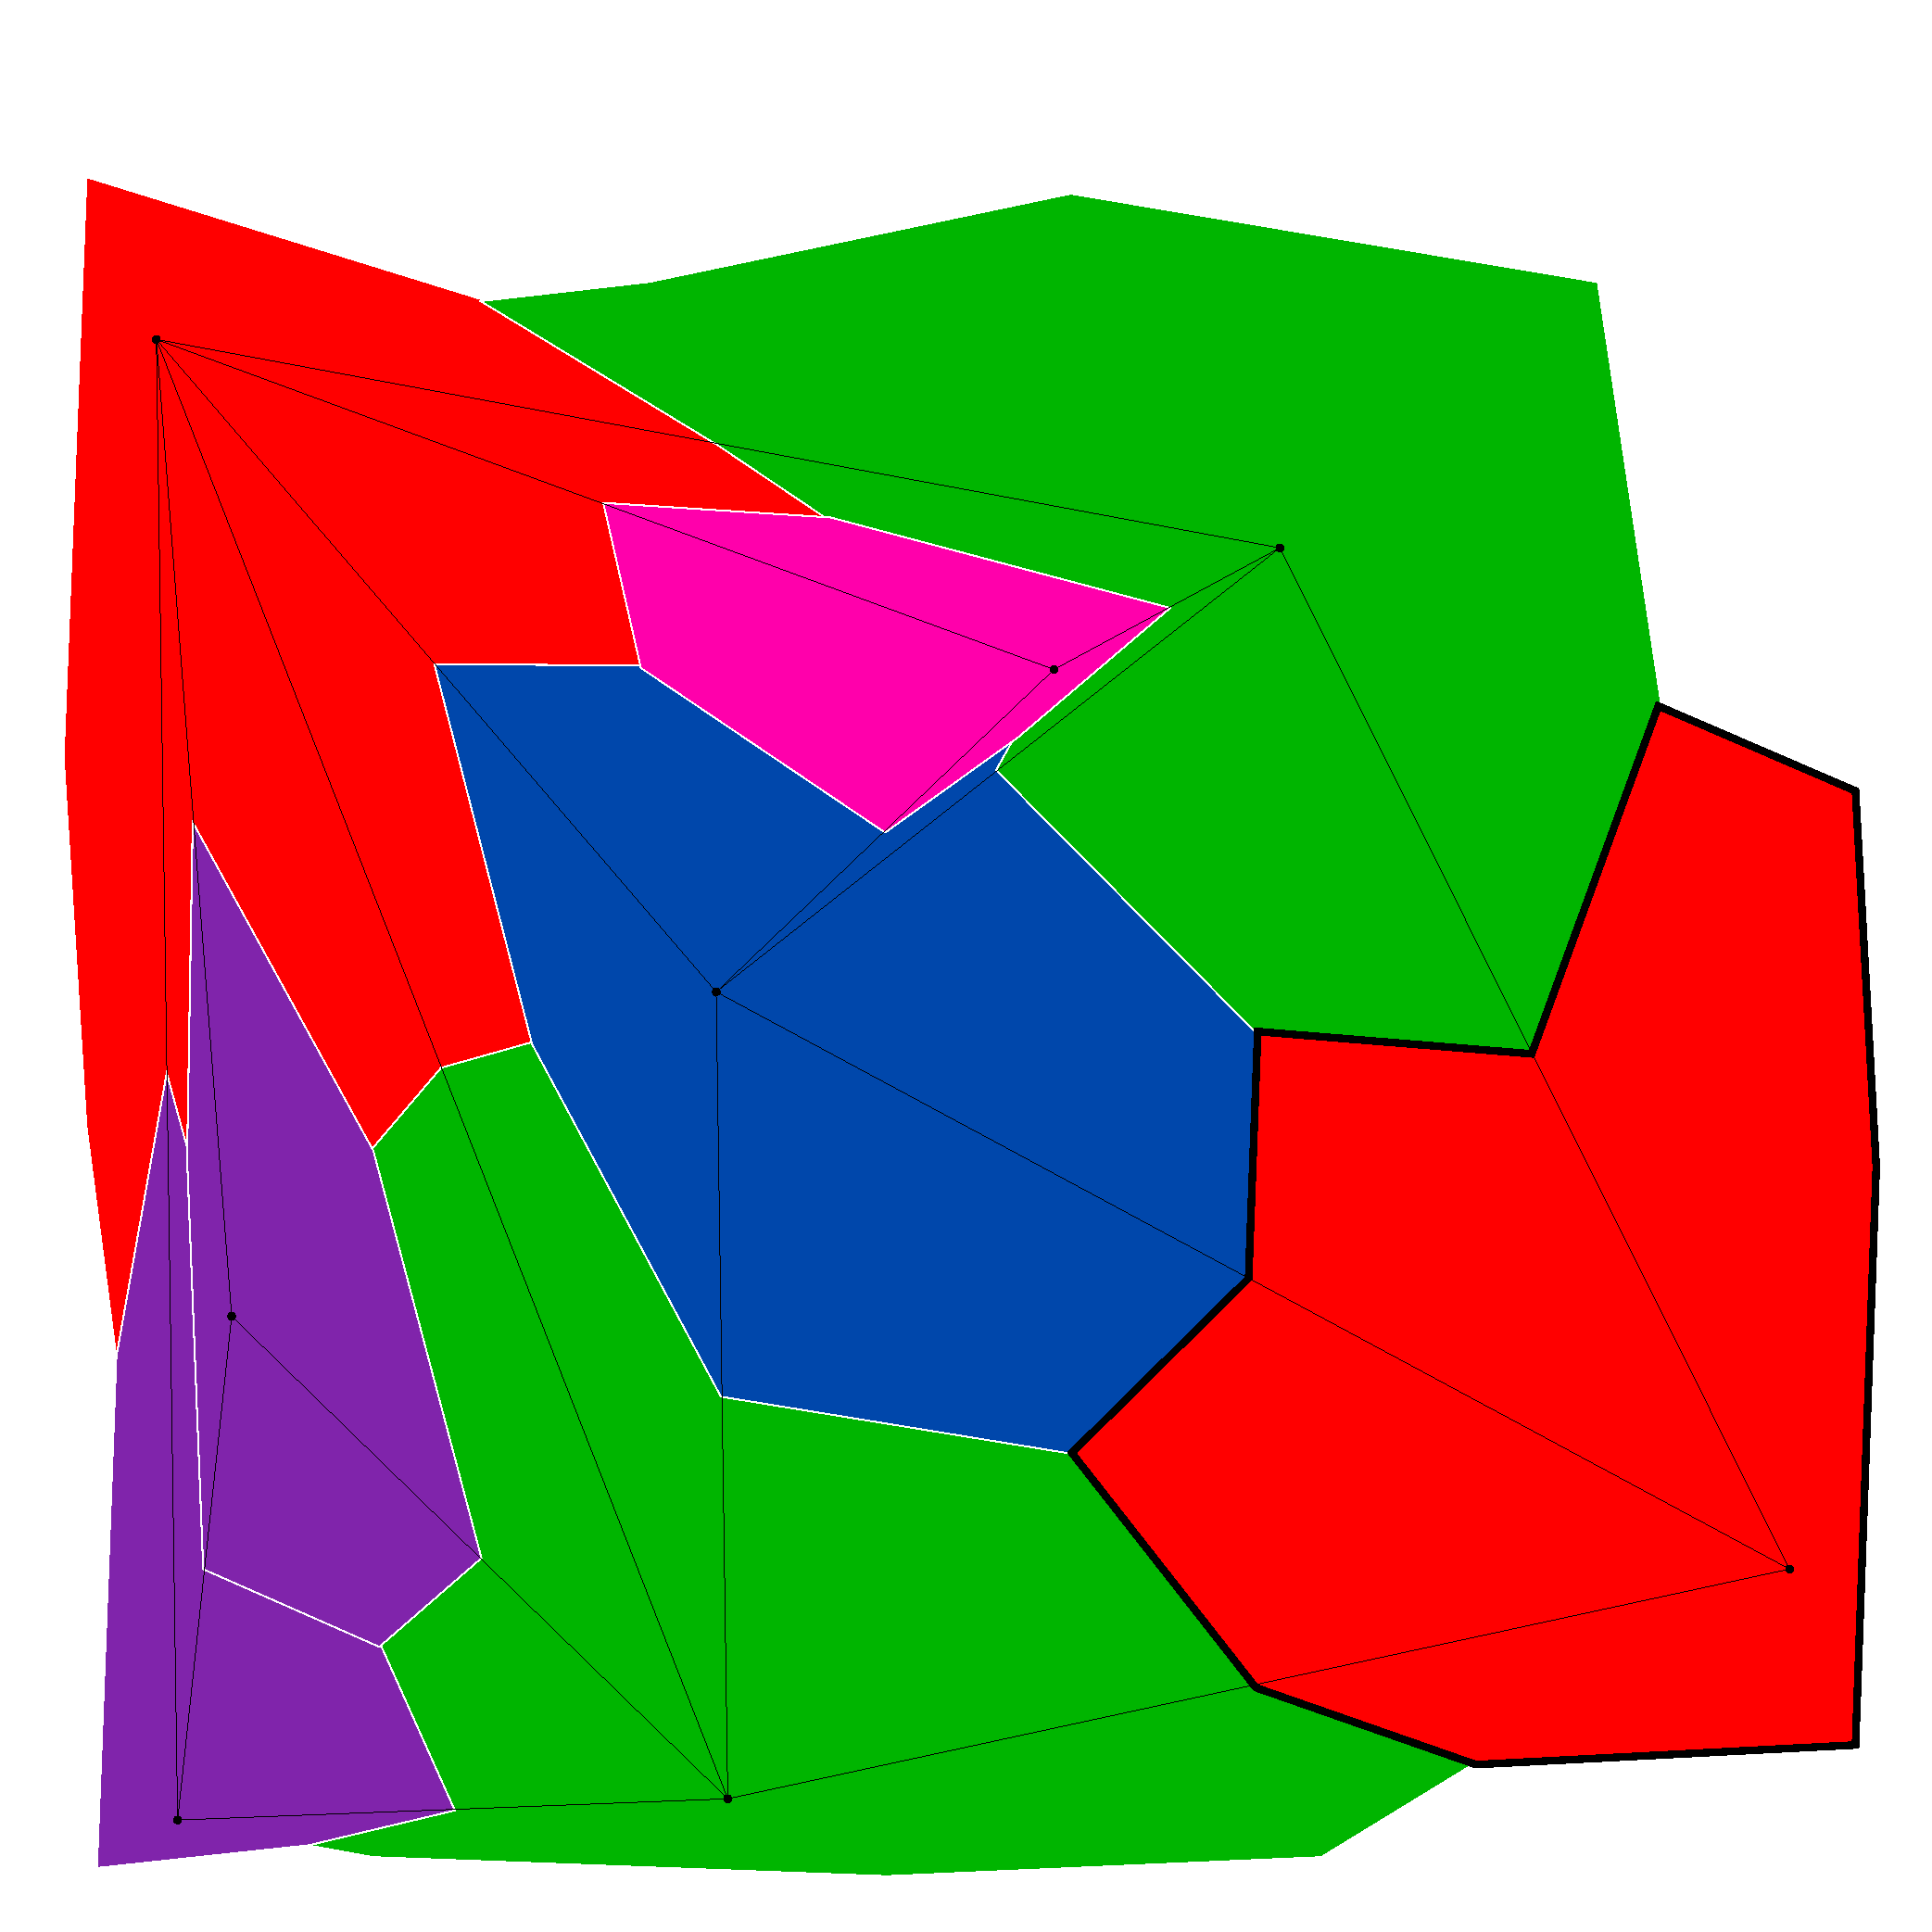
\includegraphics[width=\textwidth]{images/sequences/mac_backtracking/bt_mac_I00010}
				\caption{}
				\label{bte}
			\end{subfigure} \\
			
			\begin{subfigure}{0.18\textwidth}
				\centering
				\includegraphics[width=\textwidth]{images/sequences/mac_backtracking/bt_mac_I00012}
				\caption{}
				\label{bta}
			\end{subfigure}
			\;
			\begin{subfigure}{0.18\textwidth}
				\centering
				\includegraphics[width=\textwidth]{images/sequences/mac_backtracking/bt_mac_I00014}
				\caption{}
				\label{btb}
			\end{subfigure}
			\;
			\begin{subfigure}{0.18\textwidth}
				\centering
				\includegraphics[width=\textwidth]{images/sequences/mac_backtracking/bt_mac_I00015}
				\caption{}
				\label{btc}
			\end{subfigure}
	
			\caption{}
		\end{figure}	

	\subsection{Experimental Approach}
	
	\subsection{Results}
	
\section{Genetic Algorithm}

	\subsection{Implementation}
	Local search using a genetic algorithm involves a process similar to evolution to produce an individual that maximizes a fitness function. Since genetic algorithms are an abstraction of biological evolution, they involve some of the classic mechanisms seen in the natural world such as crossover, mutation, and survival of the fittest\cite{genetic}.
	
	The genetic algorithm begins with a population of randomly generated individuals. A selection process chooses which individuals to use for reproduction, which are weighted by their score generated the fitness function. The individuals are recombined by cross-over and the resulting individuals may be mutated depending on a small probability.
	
	To apply the genetic algorithm to the GCP we started with the genetic algorithm described in Russel and Norvig Section 4.1\cite{ai} and implemented each feature in accordance with the GCP. Our initial population consisted of $N$ randomly colored graphs. It was hard to determine what population size was the best, but it was clear that the optimal population size was related to the size of each graph and that larger graphs needed larger populations in general. $N$ was a natural number to try and it seemed to work fairly well.
	
	
	
	To select individuals for crossover we used tournament selection where two individuals were randomly selected and the one with the best fitness score  proceeded to crossover. Naturally, two tournaments were needed to get the two individuals required for crossover. In this scheme an individual could be chosen zero, one, or multiple times to participate in tournaments.
	
	The fitness function used to calculate the fitness score was essentially a penalty function because only the total number of conflicts in each individual was used to calculate the fitness score. Since this score reflected how many neighboring vertices shared colors, a large score was considered less fit and a score of zero indicated that a solution was found. 
	
	The crossover algorithm consisted of random single point crossover. To achieve this we chose a random point in each graph and swapped colors up to that point. The crossover example in Figure \ref{cross_example} looks like multi-point crossover because the vertices of the graph are unordered when crossover is performed.
	
	
	
	
	
	
	\begin{figure}[h!]
		\centering
		\begin{subfigure}{0.18\textwidth}
			\centering
			\includegraphics[width=\textwidth]{images/sequences/genetic/genetic_I00001}
			\caption{}
			
		\end{subfigure}
		\;
		\begin{subfigure}{0.18\textwidth}
			\centering
			\includegraphics[width=\textwidth]{images/sequences/genetic/genetic_I00002}
			\caption{}
			
		\end{subfigure}
		\;
		\\
		\begin{subfigure}{0.18\textwidth}
			\centering
			\includegraphics[width=\textwidth]{images/sequences/genetic/genetic_I00003}
			\caption{}
			
		\end{subfigure}
		\;		
		\begin{subfigure}{0.18\textwidth}
			\centering
			\includegraphics[width=\textwidth]{images/sequences/genetic/genetic_I00004}
			\caption{}
			
		\end{subfigure}
		
		\caption{Simple example of crossover where (a) and (b) are the parents and (c) and (d) are the offspring.}
		\label{cross_example}
	\end{figure}
	
	After crossover we immediately mutated each individual which consisted of selecting each vertex and randomly changing it depending on a mutation rate defined as $1/N$. This mutation rate was chosen because it seemed to minimize the number of iterations to find a solution. This number proved to be very specific and any deviation would negatively affect the performance of the algorithm considerable. 
	
	Once we had the new individuals we inserted them into the new population. We used pure insertion meaning that each generation was composed entirely of new individuals produced by crossover. This was later understood to be a poor choice, but it did work for this application. 
	
	This process of selection, crossover, mutation, and reinsertion was repeated until an individual with zero conflicts was found or a predefined limit on the number of generations allowed was reached. In Figure \ref{genetic_flow} a flow graph showing the general flow of our genetic algorithm. It can be seen that the population is initialized outside of the main loop. 
	
	\begin{figure}[h!]
		\centering
		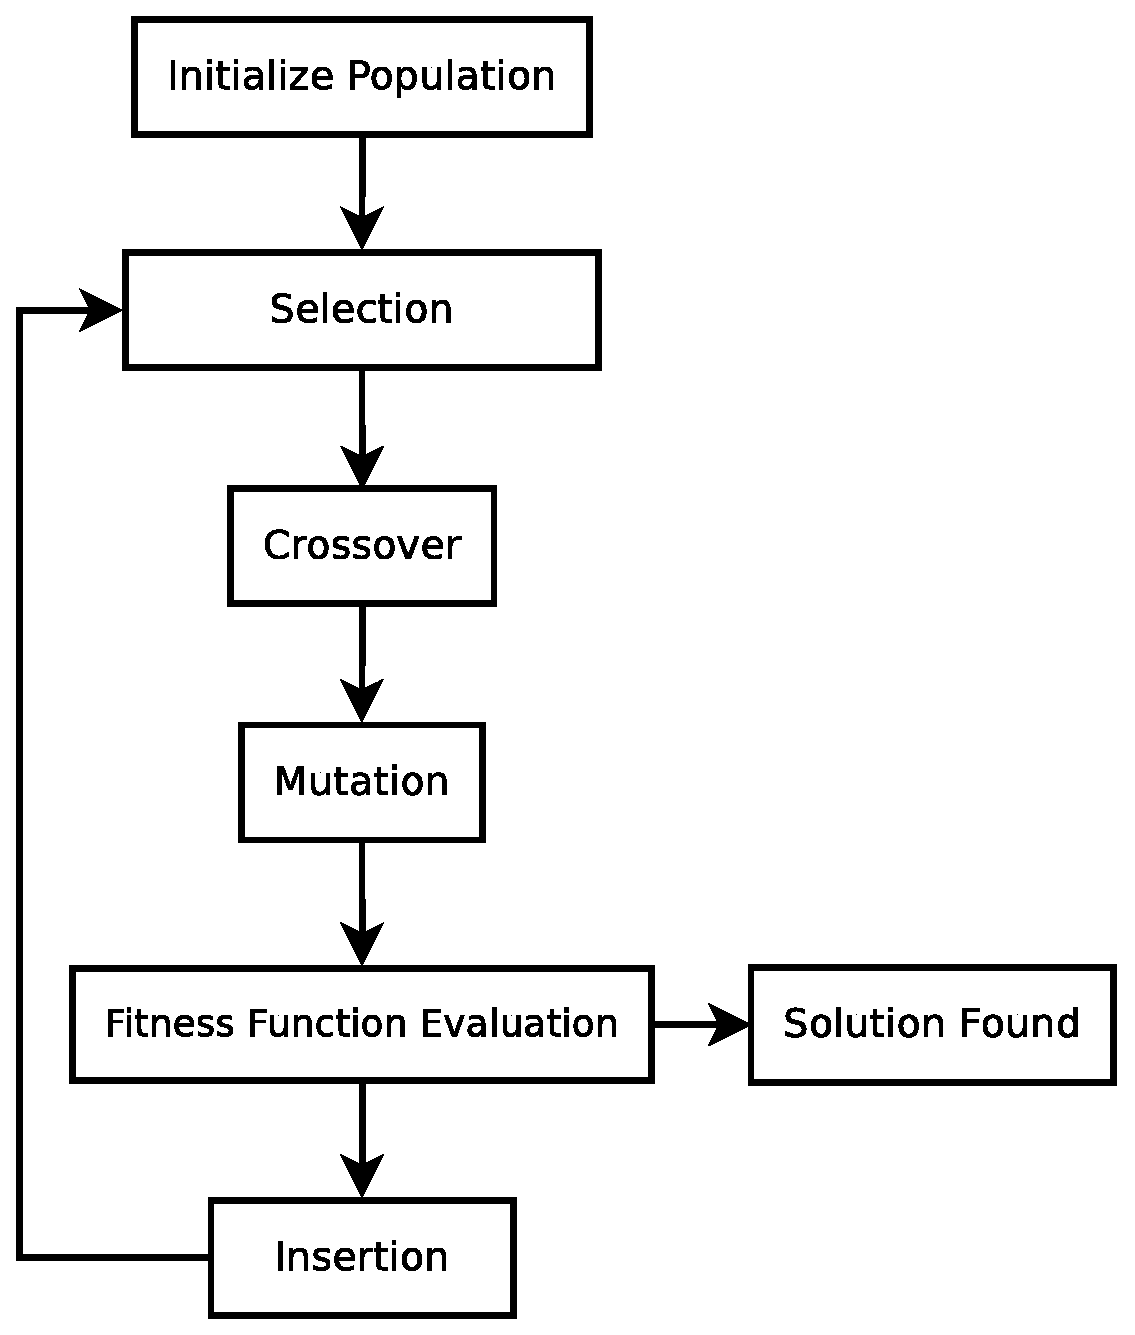
\includegraphics[width=0.45\textwidth]{images/genetic_flo}
		\caption{Flow graph of our genetic algorithm.}
		\label{genetic_flow}
	\end{figure}
	
	\subsection{Experimental Approach}
	To gauge the performance of the algorithm we will run the algorithm on graph sizes $N = (10, 20, ..., 100)$ with 20 runs of each different graph size. The metrics that will be used are number of generations, number of writes, and number of reads.
	
	The most obvious metric to use was number of generations because it tells you how many steps it took to find a solution. It was used to see how performance changed as $N$ increased and to compare the relative difficulty of graphs of the same size. Another added benefit of this metric was that it was used to find the optimal population size and mutation rate. The drawback of this metric was that it did not take into account the increased computation needed for larger graphs.
	
	One way we accounted for the increased computation time needed for larger graphs was to count the number of times we check the color of a graph vertice. This scaled with the size of the graph for two reasons. One was that each time we checked the fitness of a graph we had to read each nodes color and, as the graph got bigger, more nodes had to be read. The other reason is that, since our population is of size $N$, we have to check more graphs as the population size grows. We called this metric \texttt{num\_reads}
	
	The other way we accounted for the increased computation time needed for larger graphs was to count the number of times we change the color of a graph vertice. This metric scaled with the size of the graph for the same reasons as number of reads.
	
	\subsection{Results}
	\begin{figure}[h!]
		\centering
		\includegraphics[width=0.80\textwidth]{../results_5/genetic/genetic_performance}
		\caption{Logarithmic plot describing the performance of the genetic algorithm vs. the number of vertices. The shaded regions represent the minimum and maximum values of each quantity.}
		\label{genetic_Performance}
	\end{figure}
	
	Figure \ref{genetic_Performance} shows our metrics on a logarithmic plot. There are several points of interest on this graph. The first is how the number of generations increase as $N$ increases. We can deduce from the slope of the lines that this algorithm runs in exponential time, thought it is still much faster than a brute force approach. We can further deduce that the number of generations increases at $\mathcal{O} (e^{Na})$ where $a$ represents the slope of the line in a logarithmic plot. By deduction we can see that  $a<1$.
	
	The other points of interest are the number of reads and writes. It can be seen that the slope of the line is a little more steep than the number of generations. This is as expected because the population size increases as $N$ increases and therefore causes the number of reads and writes to grow. Even with these setbacks read and write still managed to run in approximately  $\mathcal{O} (e^{Nb})$ where $b$ represents the slope of the line in a logarithmic plot. By deduction we can see that the slope is greater than that of the number of generations and therefore $a<b$. Additionally we can see that the slope is less than one so we can further constrict b to $a<b<1$. 
\section{Comparing Algorithm Performance}
	
	\subsection{Experimental Approach}
	
	\subsection{Results}
	
	
\section{Summary}

	




	%\bibliographystyle{apj}
	\bibliographystyle{unsrt}
	
	\bibliography{sources}
\end{document}
